\documentclass[10pt,letterpaper,spanish]{article}
\usepackage{setspace}
\setstretch{1.15}

\usepackage{bbm}
\usepackage{geometry} 
\geometry{letterpaper}
\usepackage[spanish]{babel}
\usepackage{graphicx}

\usepackage[utf8]{inputenc}
%\pagestyle{myheadings}
\usepackage{verbatim}  
\usepackage{enumerate}

%\usepackage{subfig}
\usepackage{fancyhdr} 
\pagestyle{fancy} 
%\usepackage{multicol}
%\usepackage{rotating}
\usepackage{amsmath, amsthm, amssymb}
\usepackage{lscape}
\usepackage{marvosym} % Allows the use of symbols
\usepackage{float}
\usepackage{cite}
\usepackage{bibentry}
\usepackage{appendix}
\bibliographystyle{plain}
\usepackage{hyperref}
\usepackage[labelsep=period]{caption}
%\usepackage{caption}
%\usepackage[framed,numbered]{mcode}

\addto\captionsspanish{\renewcommand{\figurename}{Imagen}}
\addto\captionsspanish{\renewcommand{\tablename}{Tabla}}
\addto\captionsspanish{\renewcommand\listfigurename{Índice de imágenes}}
\addto\captionsspanish{\renewcommand\listtablename{Índice de tablas}}
%\addto\captionsspanish{\renewcommand{\captionfont}{\tt}}

\renewcommand{\headrulewidth}{.1pt} 
\renewcommand{\footrulewidth}{.1pt}

\fancyhead[L]{\scshape Christopher Lazarus García}
\fancyhead[C]{PETRUS}
\fancyhead[R]{\scshape Carlos Petricioli Araiza}
%\fancyfoot[L]{Izq}
%\fancyfoot[R]{Dere}

%%%% BASH
\usepackage{xcolor}
\usepackage{listings}
\lstset{
  basicstyle=\ttfamily,
  showstringspaces=false,
  commentstyle=\color{red},
  keywordstyle=\color{blue}
}

\begin{document}

\thispagestyle{plain}
\begin{center}
\scshape \Large Datatón: Predicción espacial de delitos en Zapopan\footnote{Reporte ejecutivo del proyecto: Predicción espacial de delitos en Zapopan del equipo PETRUS.
\\ Agradecemos el apoyo y comentarios de todos nuestros colaboradores del programa: \href{http://dssg.uchicago.edu}{\textit{Data Science for Social Good (DSSG)}}.
\\ Esta versión: \today.}

\bigskip
\large \scshape Carlos Petricioli Araiza\footnote{ \href{mailto:carpetri@gmail.com}{\Letter \ carpetri@gmail.com} }  \hfill Christopher Lazarus García
\footnote{ \href{mailto:clazarusg@gmail.com}{\Letter \ clazarusg@gmail.com} } 
\normalsize
\end{center}

\bigskip
% Tema de investigación.
% Breve síntesis metodológica.
% Resumen de resultados.
% Potencial de impacto.
% Una visualización que sustente sus resultados.
\section*{\centering  \begin{normalsize} Resumen \end{normalsize}}
\begin{quotation}
\noindent 
El \textit{tema de investigación} de este proyecto es la detección y predicción del crimen en el municipo de Zapopan. El objetivo de este proyecto es hacer una visualización espacial de los delitos en el municipio de Zapopan, Jalisco con el propósito de identificar las zonas más conflictivas y así poder hacer una predicción geográfica sobre dónde habrá más delitos y con qué caracteristicas.

La \textit{metodología} que se utiliza en este este proyecto es completamente espacial. Se consideraron los delitos 
...
Se controla por el tipo de delito y todo el análisis se realiza utilizando información sobre centros recreativos, centros de salud, información sobre las colonias,  así como información sobre parques, templos, tianguis y obras públicas. Además se consideran factores climatológicos y culturales como festividades y eventos importantes en el municipio de Zapopan.  El objetivo indirecto de este proyecto es servir de ejemplo de cómo se puede utilizar este tipo de información para el mejoramiento y desarrollo del país a partir de uso de datos abiertos.


\end{quotation}

\vfill
Tópicos: Análisis geoespacial,  Impacto Ambiental, Minería de datos, INEGI, México y Seguridad.



\newpage
\section{Introducción}

% Tema de investigación.
% Breve síntesis metodológica.
% Resumen de resultados.
% Potencial de impacto.
% Una visualización que sustente sus resultados.
% Fuente.


% Potencial de impacto (40%)
% Originalidad (30%)
% Aplicabilidad (15%)
% Visualización (15%)


\noindent  
\begin{figure}[H]
\centering
\caption{Delitos en Zapopan}
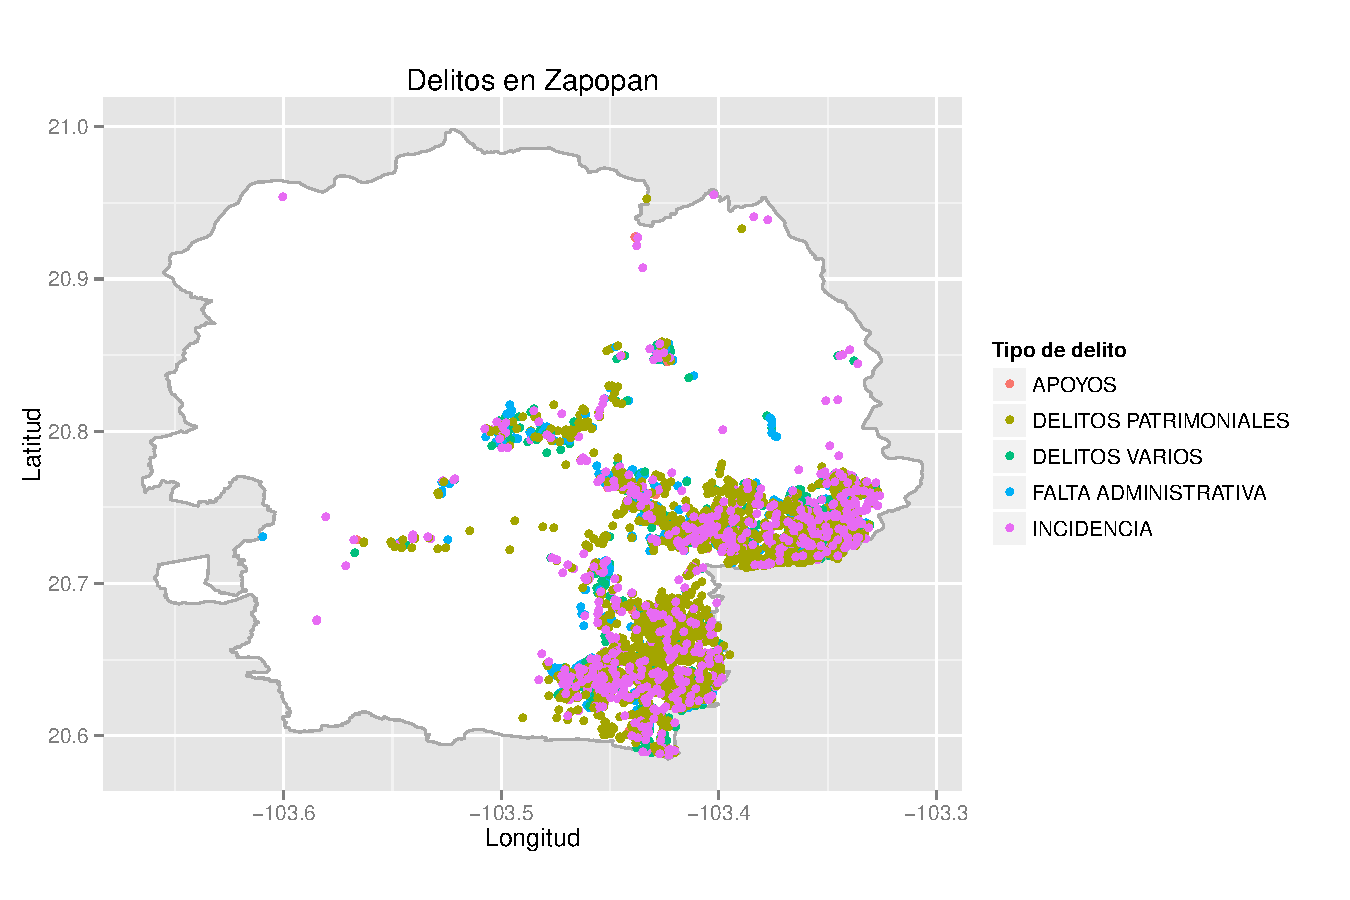
\includegraphics[width=120mm]{../../graphs/zapopan_delitos.pdf}
%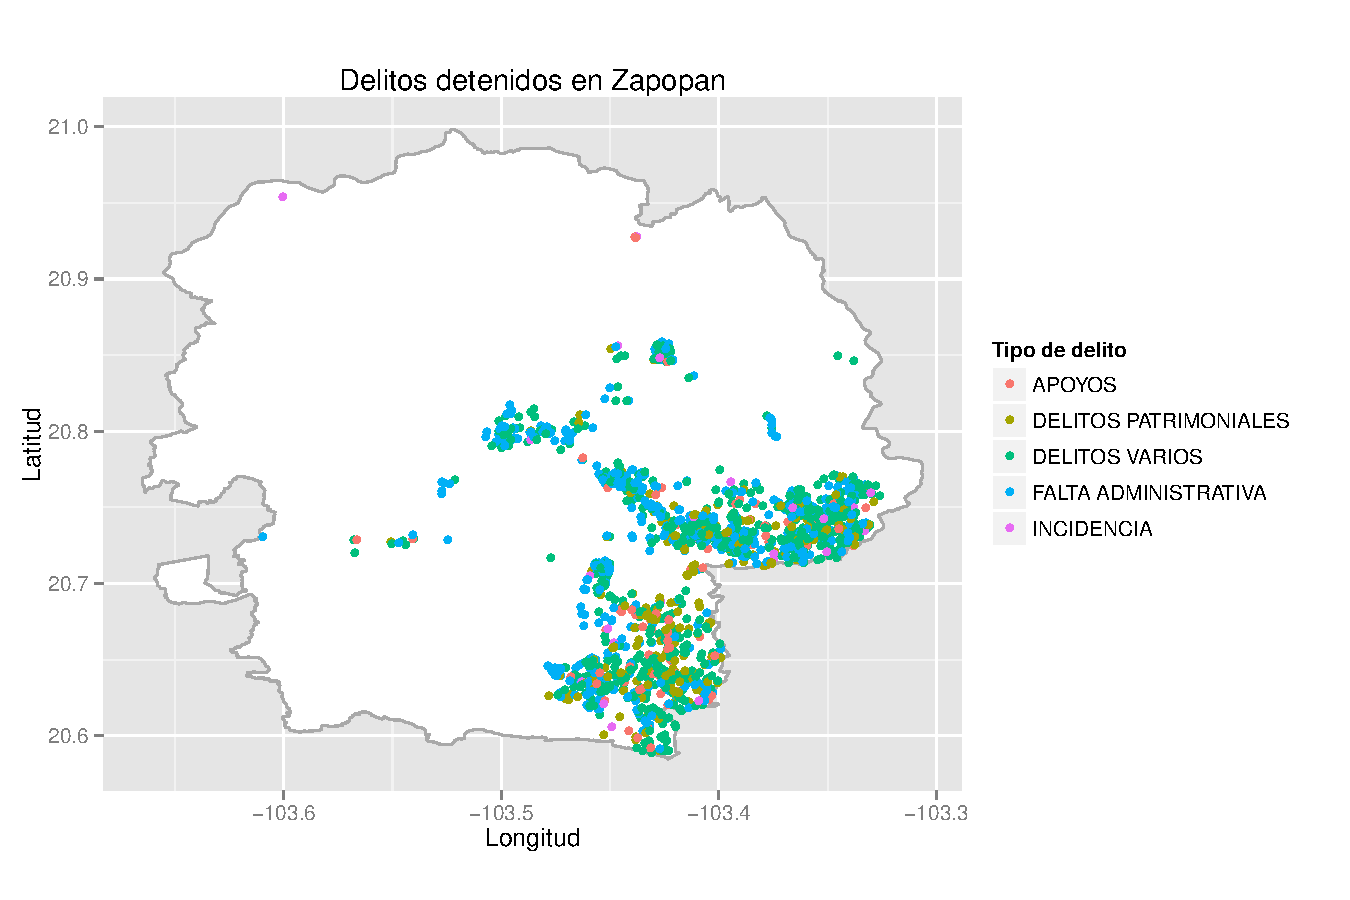
\includegraphics[width=120mm]{../../graphs/zapopan_delitos_detenidos.pdf}
\end{figure}


\begin{table}[H]
\centering
\caption{Número de delitos cometidos y detenidos} 
\begin{tabular}{lrr}
  \hline
Tipo de delito & Cometidos  \\ 
  \hline
APOYOS & 101  \\ 
  DELITOS PATRIMONIALES & 2293 \\ 
  DELITOS VARIOS & 896 \\ 
  FALTA ADMINISTRATIVA & 807 \\ 
  INCIDENCIA & 789\\ 
   \hline
\end{tabular}
\end{table}

\begin{table}[H]
\centering
\caption{Porcentaje de delitos cometidos} 
\begin{tabular}{lrr}
  \hline
Tipo de delito & \% de cometidos  \\ 
  \hline
APOYOS & 2 \\ 
  DELITOS PATRIMONIALES & 47 \\ 
  DELITOS VARIOS & 18  \\ 
  FALTA ADMINISTRATIVA & 17  \\ 
  INCIDENCIA & 16  \\ 
   \hline
\end{tabular}
\end{table}

\begin{table}[H]
\centering
\caption{Las 20 colonias más peligrosas} 
\begin{tabular}{rllr}
  \hline
 & Colonia & Tipo de delito & n \\ 
  \hline
1 & PASEOS DEL SOL & DELITOS PATRIMONIALES &  70 \\ 
  2 & TABACHINES & DELITOS PATRIMONIALES &  67 \\ 
  3 & SAN JUAN DE OCOTAN & FALTA ADMINISTRATIVA &  65 \\ 
  4 & ARBOLEDAS & DELITOS PATRIMONIALES &  57 \\ 
  5 & CALMA LA & DELITOS PATRIMONIALES &  49 \\ 
  6 & CABECERA MUNICIPAL & FALTA ADMINISTRATIVA &  45 \\ 
  7 & JARDINES VALLARTA & DELITOS PATRIMONIALES &  39 \\ 
  8 & SAN JUAN DE OCOTAN & DELITOS VARIOS &  39 \\ 
  9 & ESTANCIA LA & DELITOS PATRIMONIALES &  38 \\ 
  10 & MIRAMAR & DELITOS PATRIMONIALES &  38 \\ 
  11 & ARCOS DE ZAPOPAN & DELITOS PATRIMONIALES &  37 \\ 
  12 & COLLI EL & DELITOS PATRIMONIALES &  37 \\ 
  13 & CABECERA MUNICIPAL & DELITOS PATRIMONIALES &  36 \\ 
  14 & PARAISOS DEL COLLI & DELITOS PATRIMONIALES &  36 \\ 
  15 & AGUILAS LAS & DELITOS PATRIMONIALES &  34 \\ 
  16 & CONSTITUCION & DELITOS VARIOS &  33 \\ 
  17 & CONSTITUCION & DELITOS PATRIMONIALES &  29 \\ 
  18 & ARENALES TAPATIOS & DELITOS VARIOS &  28 \\ 
  19 & CABECERA MUNICIPAL & DELITOS VARIOS &  28 \\ 
  20 & CAMICHINES VALLARTA & DELITOS PATRIMONIALES &  26 \\ 
   \hline
\end{tabular}
\end{table}

\begin{figure}[H]
\centering
\caption{Delitos en Zapopan por colonia}
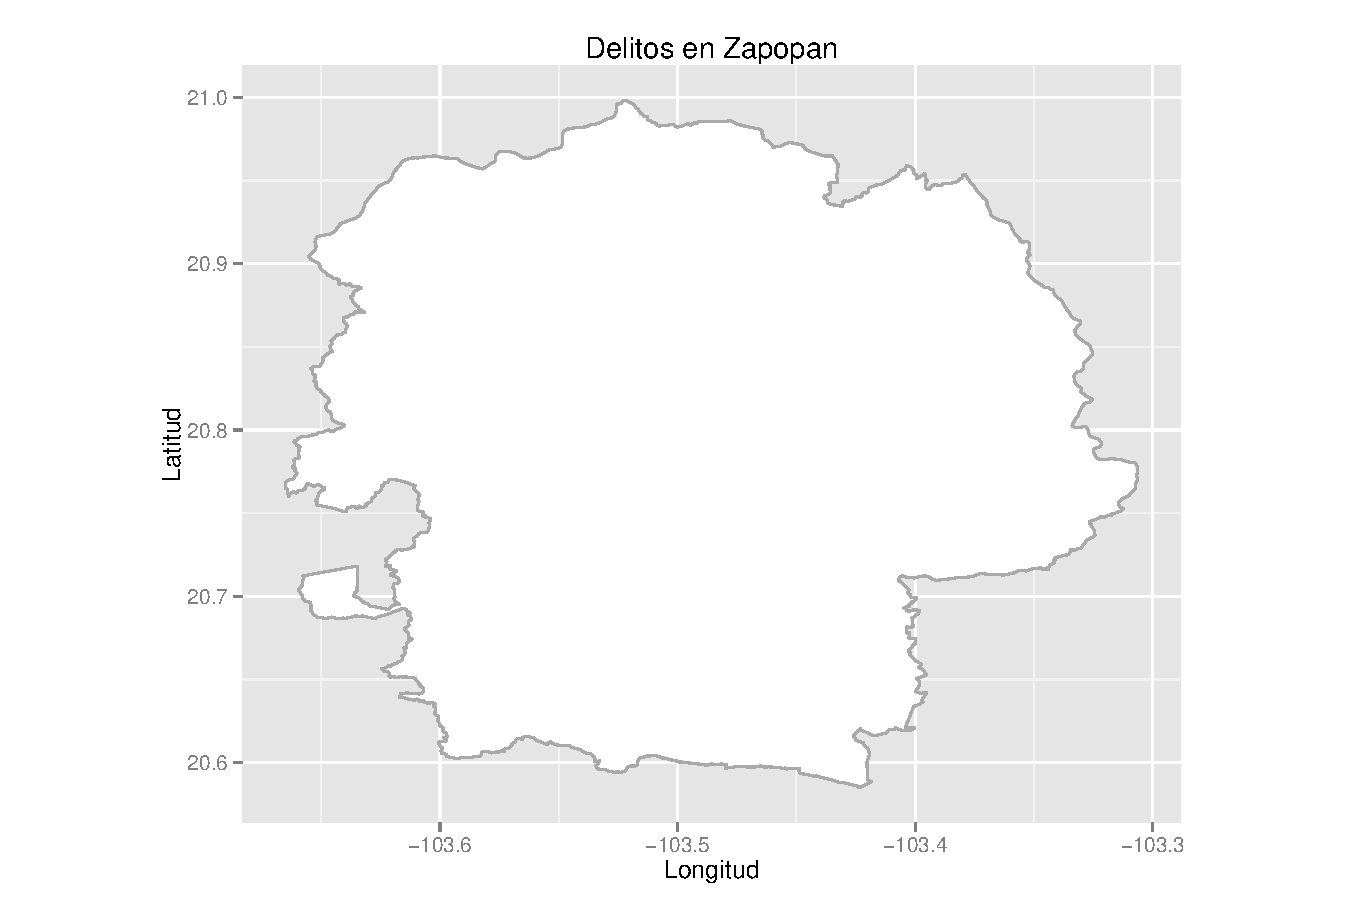
\includegraphics[width=120mm]{../../graphs/num_delitos.pdf}
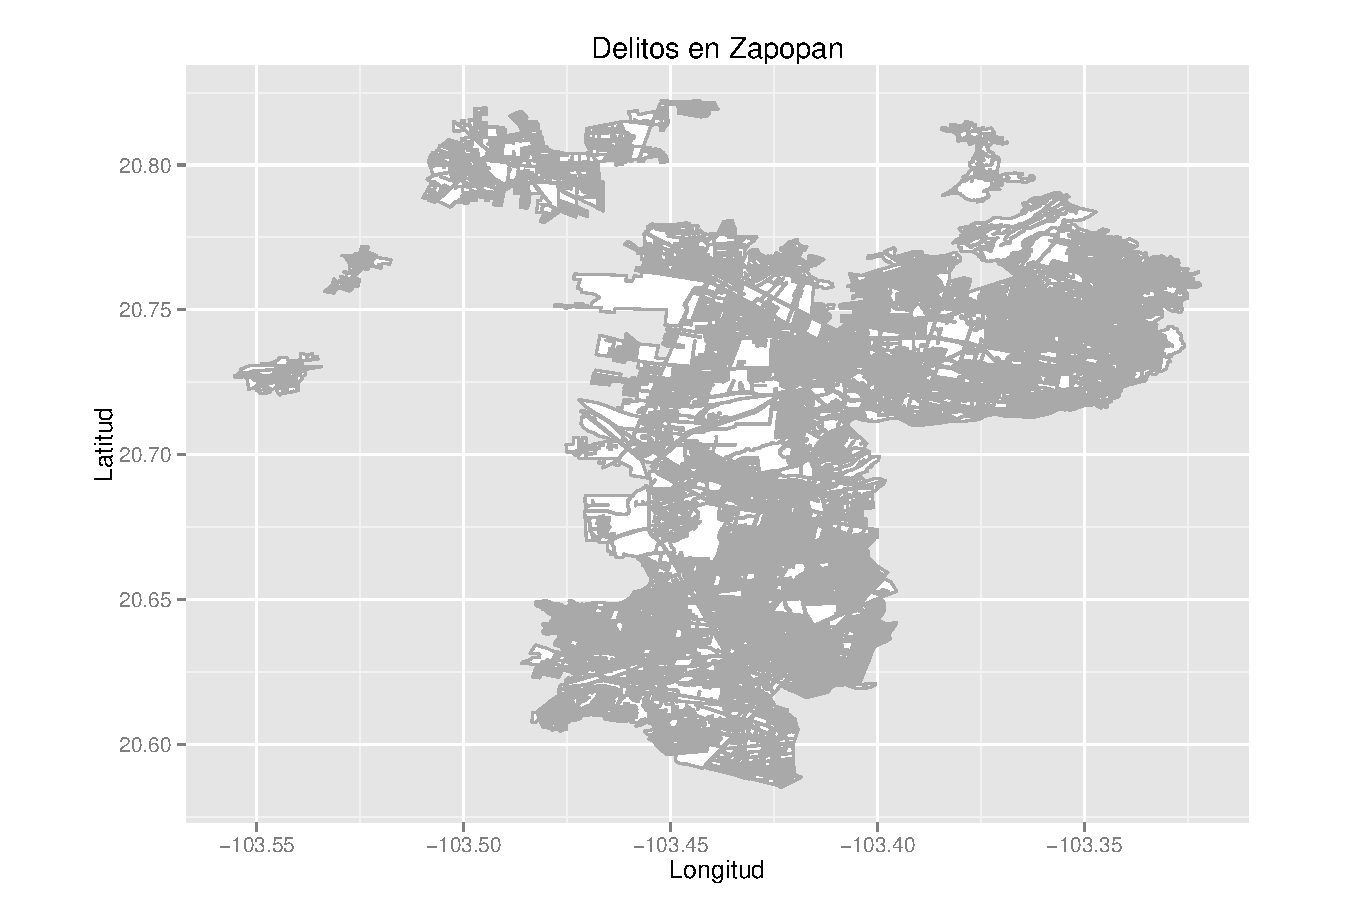
\includegraphics[width=120mm]{../../graphs/num_delitos_manz.pdf}
%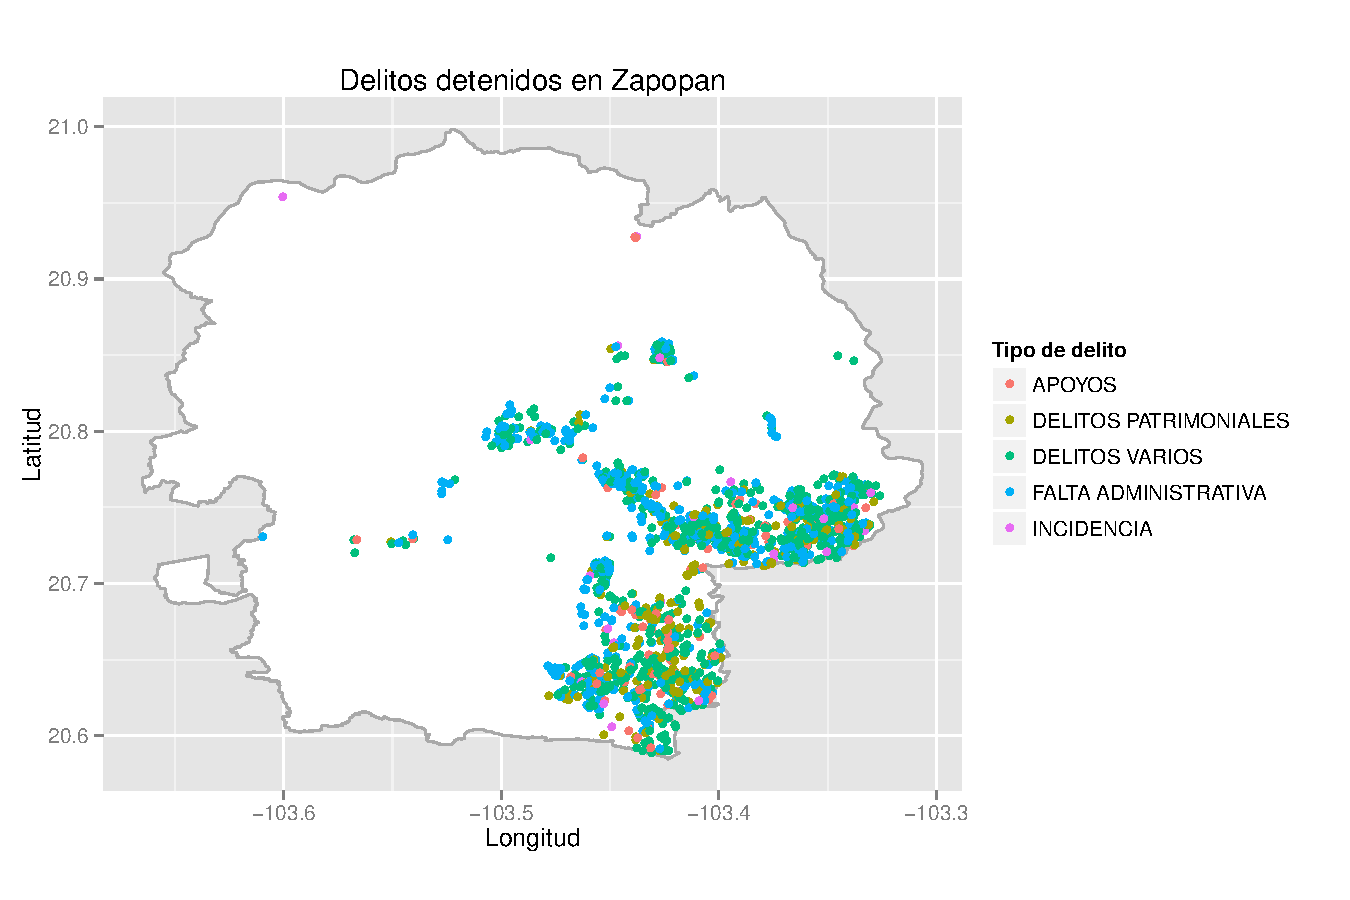
\includegraphics[width=120mm]{../../graphs/zapopan_delitos_detenidos.pdf}
\end{figure}


% latex table generated in R 3.0.3 by xtable 1.7-3 package
% Thu Jun 26 10:26:59 2014
\begin{table}[H]
\centering
\caption{Número de delitos por mes en Zapopan} 
\begin{tabular}{rr}
  \hline
mes & n \\ 
  \hline
1.00 & 1578 \\ 
  2.00 & 1543 \\ 
  3.00 & 1765 \\ 
   \hline
\end{tabular}

\end{table}


\begin{figure}[H]
\centering
\caption{Delitos en Zapopan por colonia cada mes}
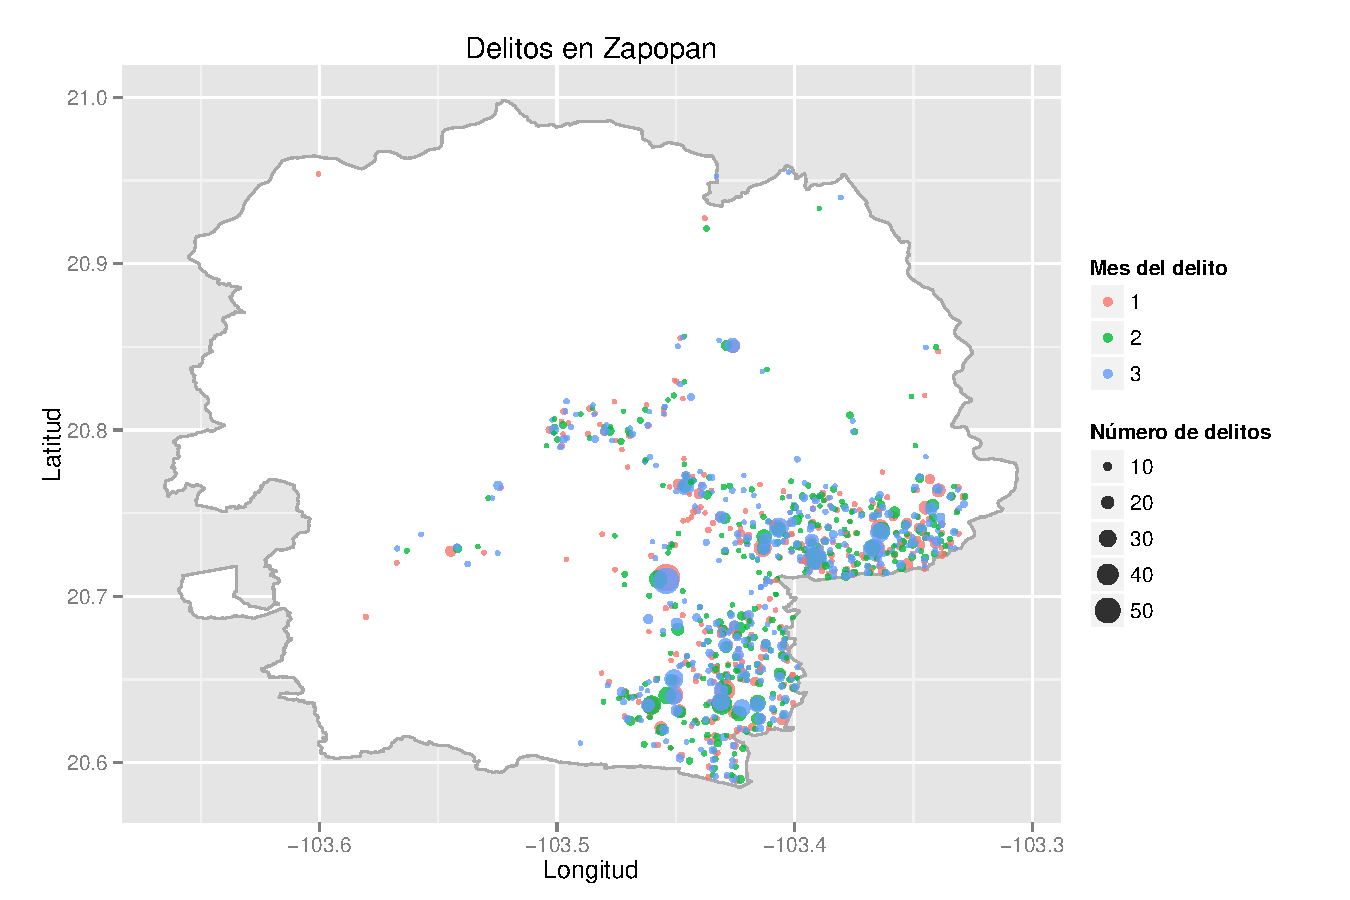
\includegraphics[width=120mm]{../../graphs/num_delitos_mes.pdf}
%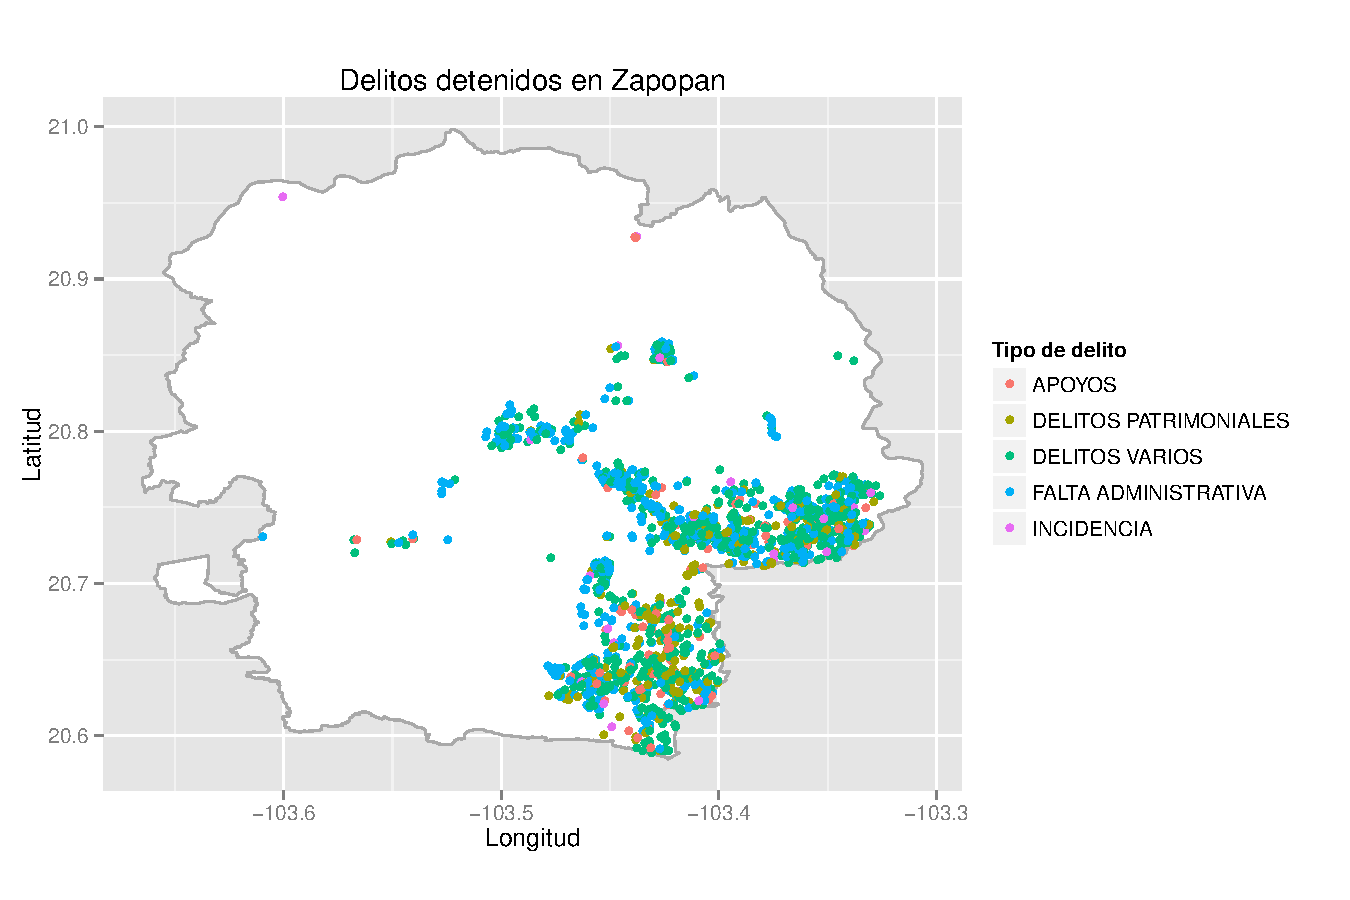
\includegraphics[width=120mm]{../../graphs/zapopan_delitos_detenidos.pdf}
\end{figure}


\begin{table}[H]
\centering
\caption{Temperatura media y delitos en Zapopan}
\begin{tabular}{lrr}
  \hline
Temperatura & Número & Proporción \\ 
  \hline
(13.3,16.9) & 980 & 20 \\ 
  (16.9,18.8) & 1122 & 23 \\ 
  (18.8,19.9) & 906 & 19 \\ 
  (19.9,20.8) & 956 & 20 \\ 
  (20.8,24.1) & 922 & 19 \\ 
   \hline
\end{tabular}
\end{table}


\begin{figure}[H]
\centering
\caption{Delitos en Zapopan por Temperatura}
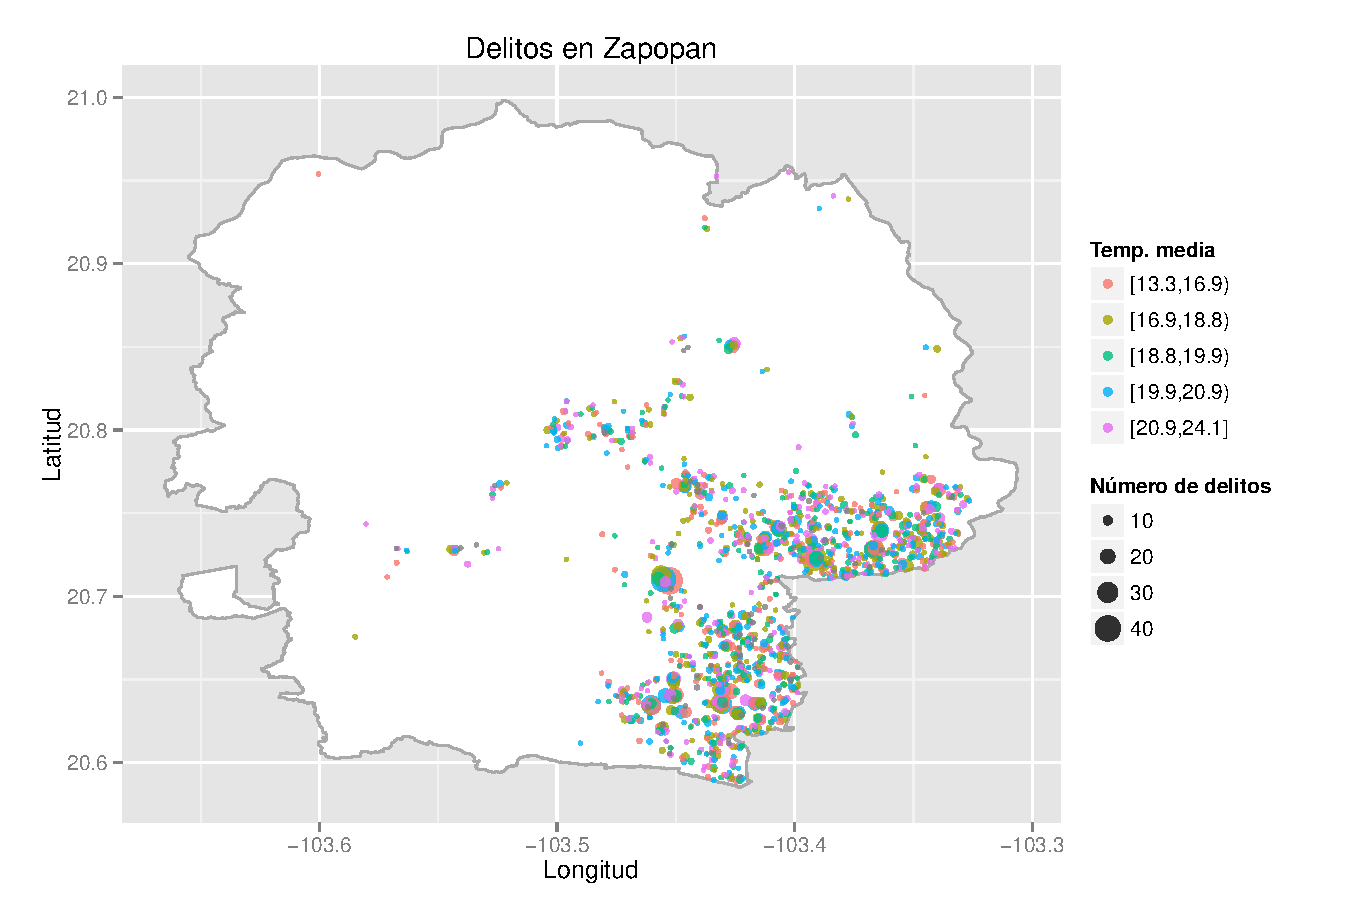
\includegraphics[width=120mm]{../../graphs/temperatura.pdf}
\end{figure}

\begin{table}[ht]
\centering
\begin{tabular}{lrrr}
  \hline
colonia & n.cometidos & n.detenidos & div \\ 
  \hline
CHAPALITA & 28 & 1 & 28 \\ 
  RESIDENCIAL VICTORIA & 21 & 1 & 21 \\ 
  LOMAS UNIVERSIDAD & 15 & 1 & 15 \\ 
  BOSQUES DEL CENTINELA & 14 & 1 & 14 \\ 
  PRADOS TEPEYAC & 14 & 1 & 14 \\ 
  JARDINES DE LA PATRIA & 13 & 1 & 13 \\ 
  LAGOS DEL COUNTRY & 13 & 1 & 13 \\ 
  VALLARTA LA PATRIA & 12 & 1 & 12 \\ 
  RESIDENCIAL PLAZA GUADALUPE & 20 & 2 & 10 \\ 
  HIGUERA LA & 8 & 1 & 8 \\ 
  HOGARES DE NUEVO MEXICO & 8 & 1 & 8 \\ 
  INDUSTRIAL BELENES NORTE & 8 & 1 & 8 \\ 
  RESIDENCIAL PONIENTE & 15 & 2 & 8 \\ 
  LOMAS DE ZAPOPAN & 29 & 4 & 7 \\ 
  ESTRADA LA & 7 & 1 & 7 \\ 
  VILLA UNIVERSITARIA & 7 & 1 & 7 \\ 
  VILLAS DE LOS BELENES & 7 & 1 & 7 \\ 
  JARDINES VALLARTA & 43 & 7 & 6 \\ 
  EUCALIPTO VALLARTA & 6 & 1 & 6 \\ 
  REAL VALLARTA & 27 & 5 & 5 \\ 
   \hline
\end{tabular}
\end{table}


\begin{figure}[H]
\centering
\caption{\textit{Heatmap} de inseguridad}
%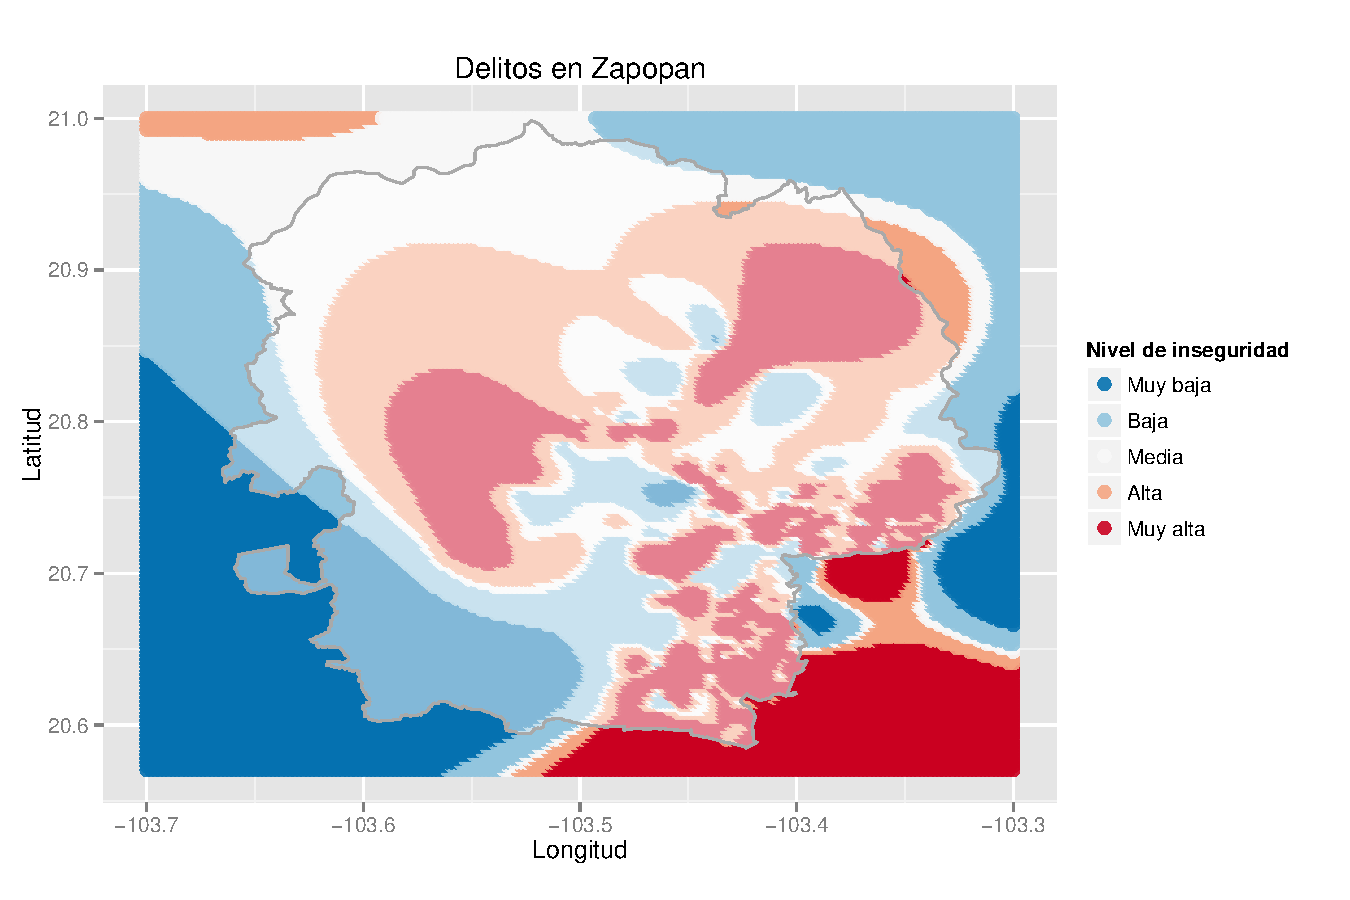
\includegraphics[width=120mm]{../../graphs/heat.pdf}
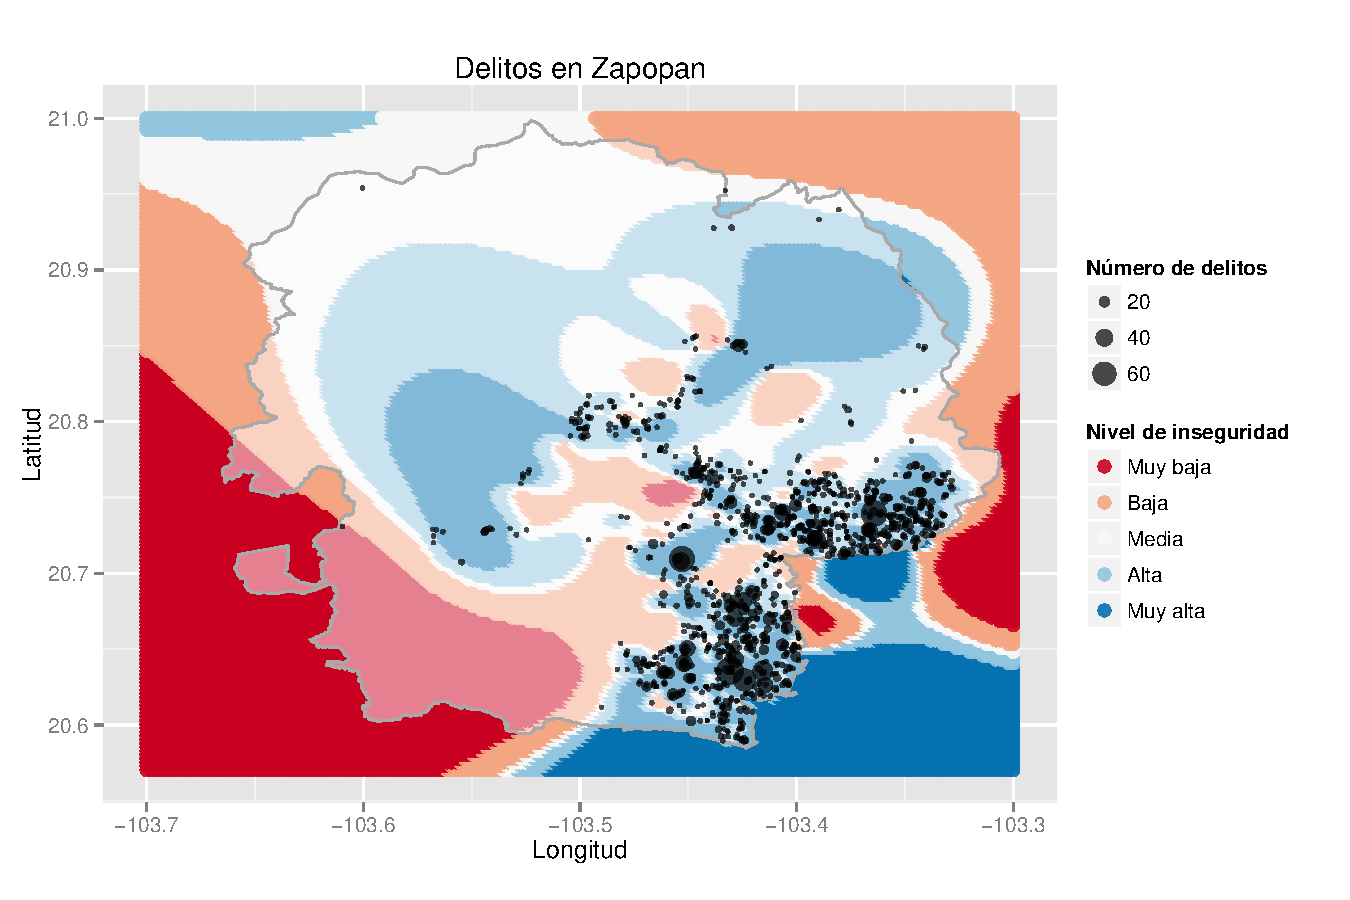
\includegraphics[width=120mm]{../../graphs/heat_y_delitos.pdf}
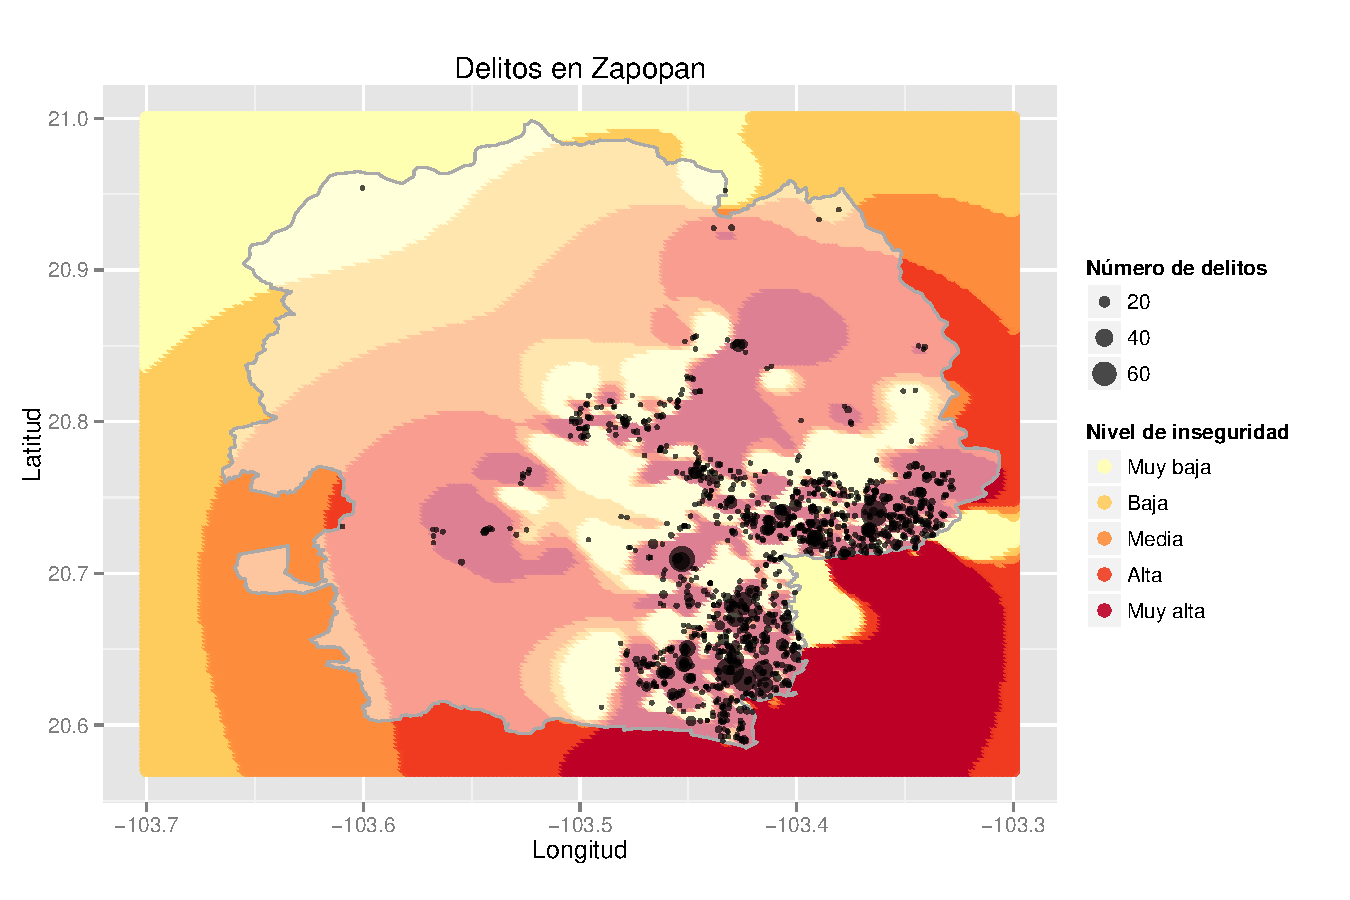
\includegraphics[width=120mm]{../../graphs/heat_y_delitos2.pdf}
\end{figure}

\begin{figure}[H]
\centering
\caption{\textit{Heatmap} de inseguridad Cometidos y Detenidos}

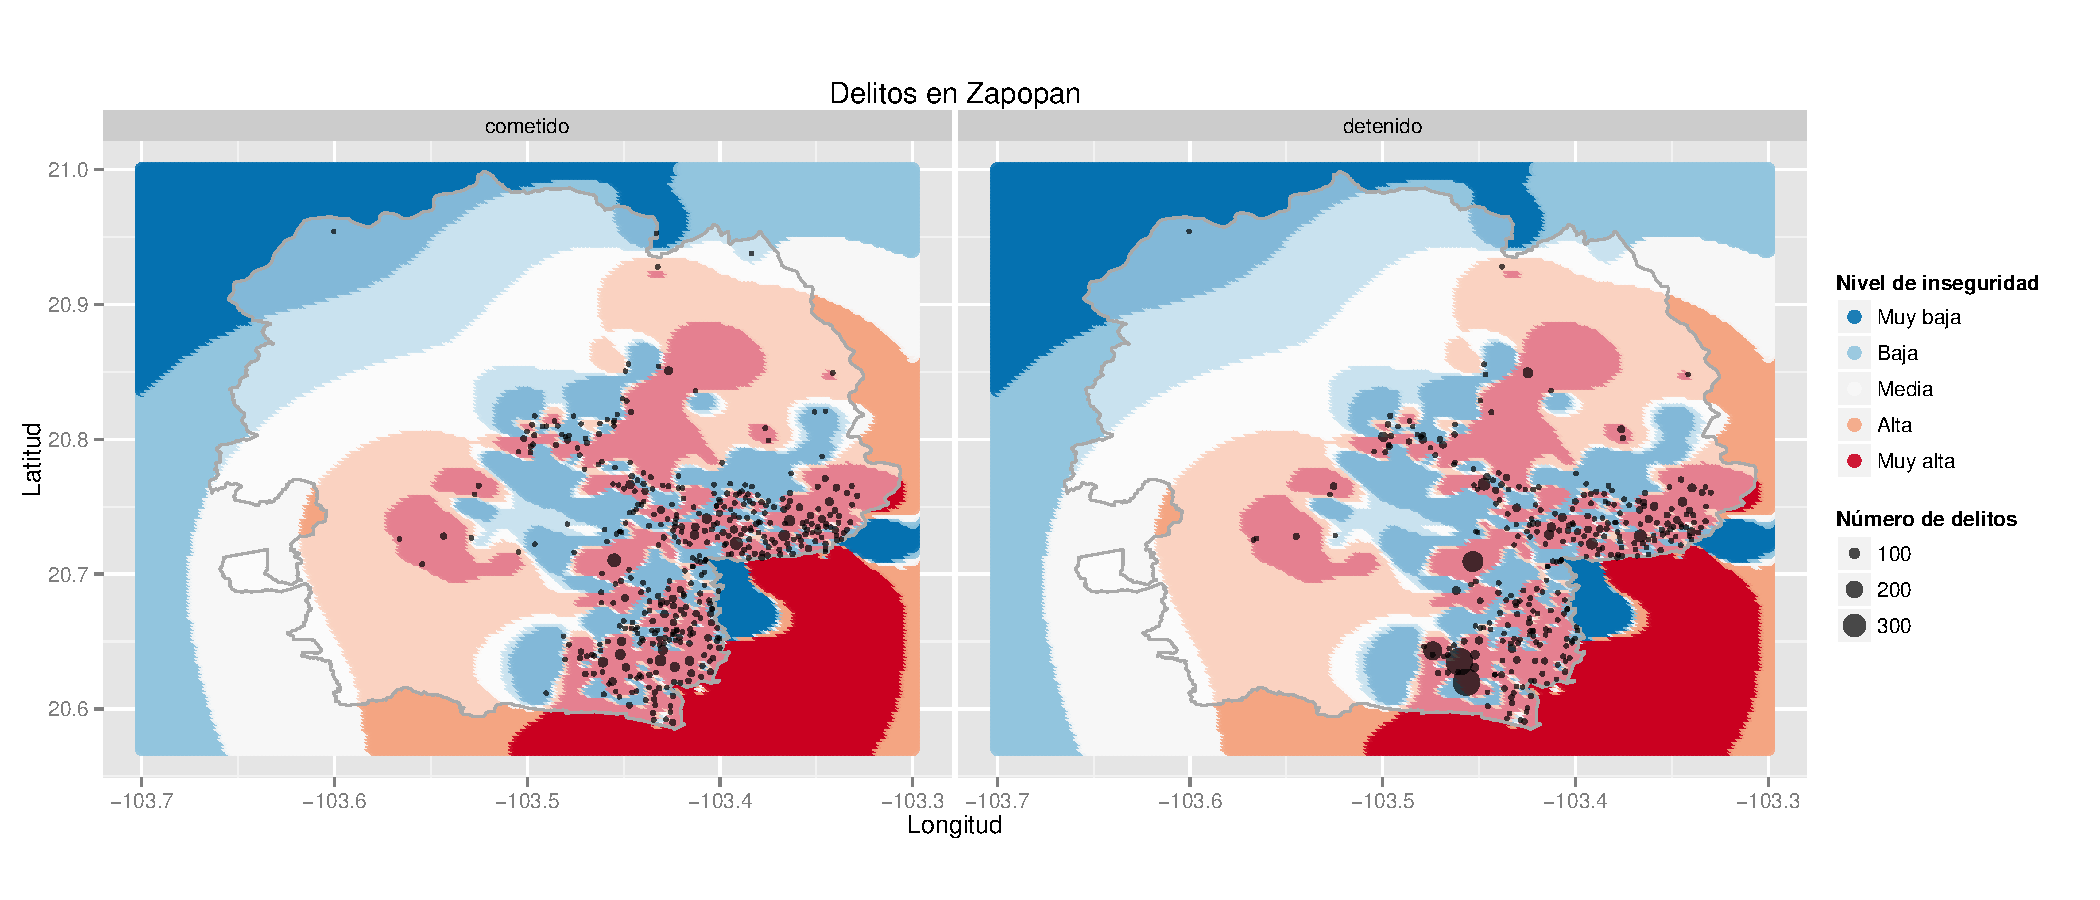
\includegraphics[width=120mm]{../../graphs/heat_facet.pdf}
\end{figure}




% \input{cap3.tex}
% \input{cap4.tex}

\appendix
% \input{anexo1.tex}

%\bibliography{biblio.bib}

\end{document}
